\begin{figure}[ht]
	\centering
	\footnotesize

	\psfrag{p1}[c][c] {$n_1$}
	\psfrag{p2}[c][c] {$n_2$}
	\psfrag{p3}[c][c] {$n_3$}
	\psfrag{p4}[c][c] {$n_4$}
	\psfrag{p5}[c][c] {$n_5$}
	\psfrag{pn2}[c][c] {$n_{n-2}$}
	\psfrag{pn1}[c][c] {$n_{n-1}$}
	\psfrag{pn}[c][c] {$n_{n}$}

	\psfrag{um1}[c][c] {$u_{-1}$}
	\psfrag{u0}[c][c] {$u_0$}
	\psfrag{u1}[c][c] {$u_1$}
	\psfrag{u2}[c][c] {$u_2$}
	\psfrag{u3}[c][c] {$u_3$}
	\psfrag{u4}[c][c] {$u_4$}
	\psfrag{u5}[c][c] {$u_5$}
	\psfrag{un2}[c][c] {$u_{n-2}$}
	\psfrag{un1}[c][c] {$u_{n-1}$}
	\psfrag{un}[c][c] {$u_{n}$}

	\psfrag{up0}[l][l] {$u'(0)=0$}
	\psfrag{uL}[r][r] {$u(1)=0$}

	\psfrag{e1}[c][c] {$e_1$}
	\psfrag{e2}[c][c] {$e_2$}
	\psfrag{e3}[c][c] {$e_3$}
	\psfrag{e4}[c][c] {$e_4$}
	%\psfrag{e5}[c][c] {$e5$}

	\psfrag{x}[c][c] {$x$}
	\psfrag{xl}[c][c] {$x_{e}^{\text{left}}$}
	\psfrag{xr}[c][c] {$x_{e}^{\text{right}}$}

	\psfrag{xm1}[c][c] {$\mathleftghost \ x_{-1}$}
	\psfrag{x0}[c][c] {$x_0$}
	\psfrag{x1}[c][c] {$x_1$}
	\psfrag{x2}[c][c] {$x_2$}
	\psfrag{x3}[c][c] {$x_3$}
	\psfrag{x4}[c][c] {$x_4$}
	\psfrag{xn2}[c][c] {$x_{n-2}$}
	\psfrag{xn1}[c][c] {$x_{n-1}$}
	\psfrag{xn}[c][c] {$x_{n}$}

	\psfrag{l}[c][c] {$l=1$}

	\psfrag{omge}[c][c] {$\Omega^{e}$}
	\psfrag{omga}[c][c] {$\Omega$}

	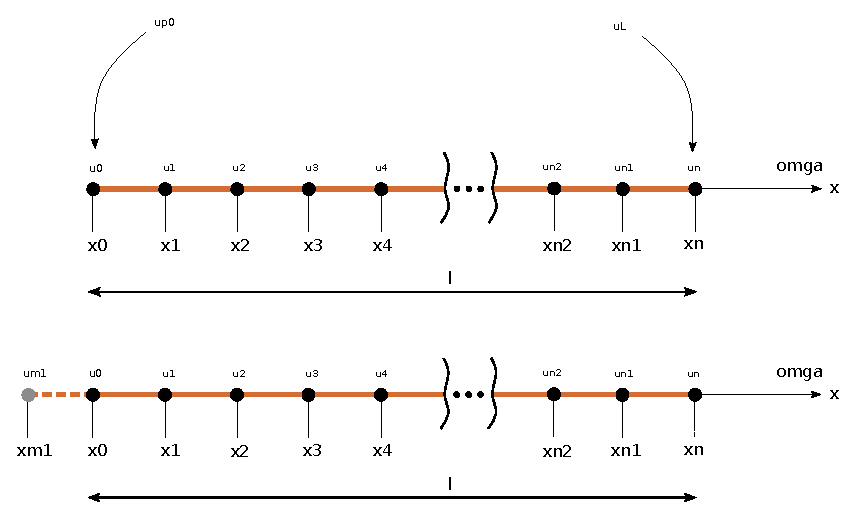
\includegraphics[width=0.9\textwidth]{discretizeGhostLeft.eps}

	\caption{Discretization of domain $\Omega$ with $n+1$ points: From $x_{0}$ to $x_{n}$.
		Ghost point $x_{n+1}$ is located on the left boundary $\partial\Omega_{L}$.}
	\label{\LABEL}
\end{figure}